\section{Implementation}
\begin{figure}
    \centering 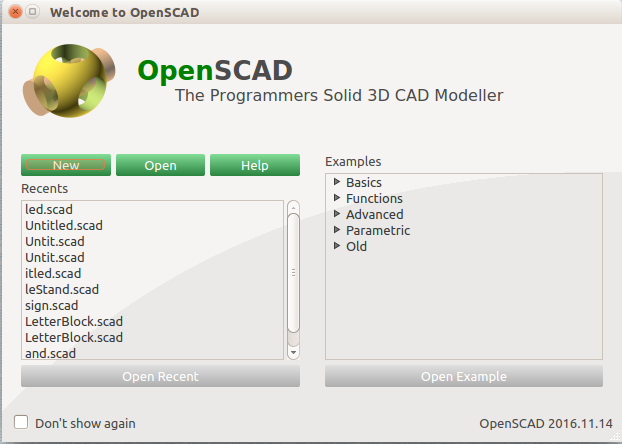
\includegraphics[width=0.7\linewidth]{images/output/1.png}
    \caption{StartUp Screen for OpenSCAD}
    \label{fig:1}
\end{figure}
\subsection{Multithreading}
In order to understand how we have attempted to implement multithreading for geometric rendering we need to understand the problem in substantial detail.\\
Even though it has been mentioned before profoundly, we feel the need the reiteration of what OpenSCAD is and how it achieves its goals. OpenSCAD is a 3D modeler i.e. it creates 3D models. The user interaction is done through a scripting language. This language describes the object(s) that the user wishes to create. This system has been put in place for the following reasons:
\begin{itemize}
	\item The fundamental geometric constructs of general purpose programming languages are too complex for an avergae computer user to learn and master. Even though ultimately, these constructs are being used to make everything in OpenSCAD but it is very difficult to expose the user to such tools. They are a little too fundamental and esoteric for the software to be of any help to your average modeler or designer who are unlikely to have much expertise of computer programming.\\
	That is why it becomes very important that the user is given an interface which has much less steeper learning curve than direct usage of geometric libraries. The OpenSCAD modelling language is just the interface for the job.
	\item Freedom and flexibilty of designing can be greatly compromised if only GUI constructs are used for modelling purpose. It is essential to give the user enough power to create complex and intricate designs easily without havnig to be limited by what the GUI has to offer. The modelling language, while being very intuitive is in fact very powerfull. The learning curve is much more user friendly without compromising the user's ability to make powerful designs. It saves a lot of time to use a higher abstraction of geometric constructs than to use the fundamentals them selves.\\
	The OpenSCAD modelling language thrives for the reasons any high level language thrives over a more machine related language. Time and effort of the programmer is saved and readability, portability are gained.
\end{itemize}
Here is a snapshot of the a model description using the above mentioned langauage:
\begin{figure}
    \centering 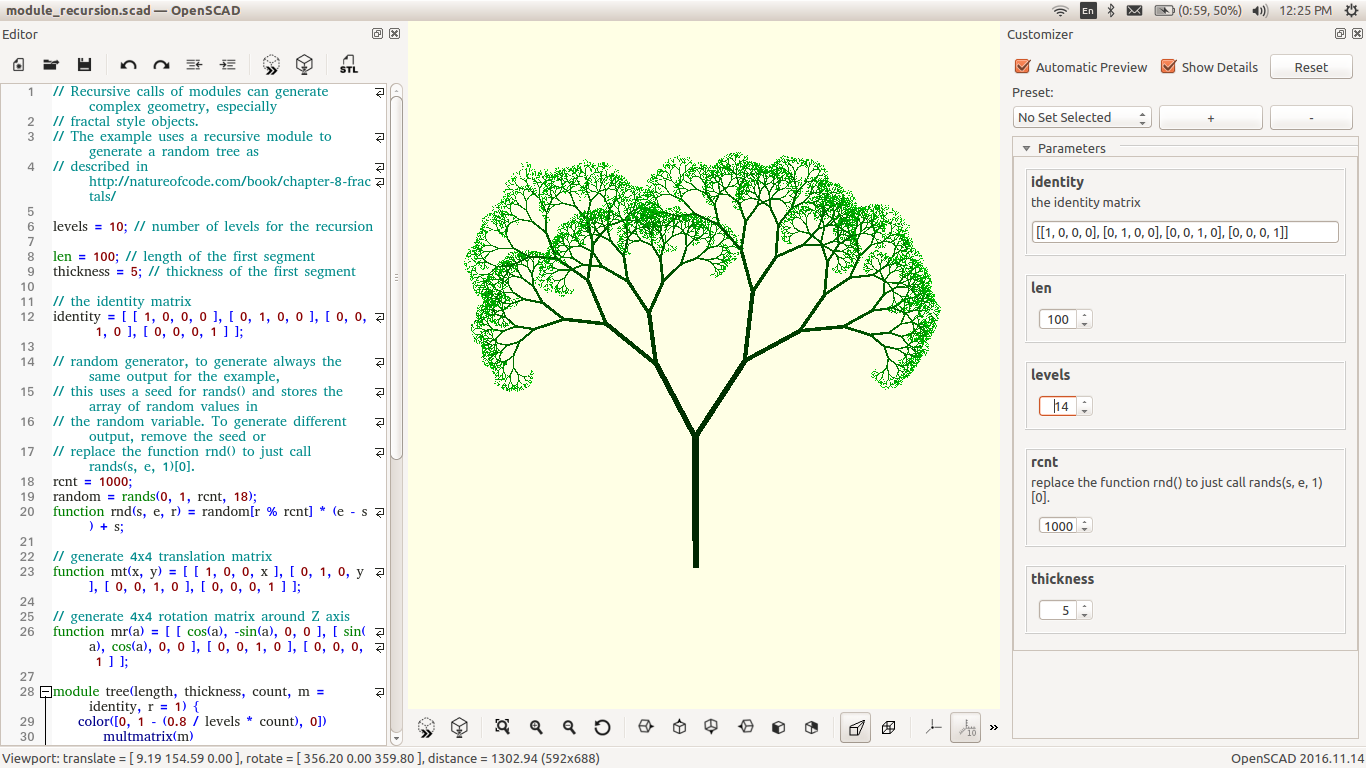
\includegraphics[width=\linewidth]{images/output/5.png}
    \caption{StartUp Screen for OpenSCAD}
    \label{fig:1}
\end{figure}
